\begin{figure}[htbp]
	\centering
	\resizebox{0.8\textwidth}{!}{%
		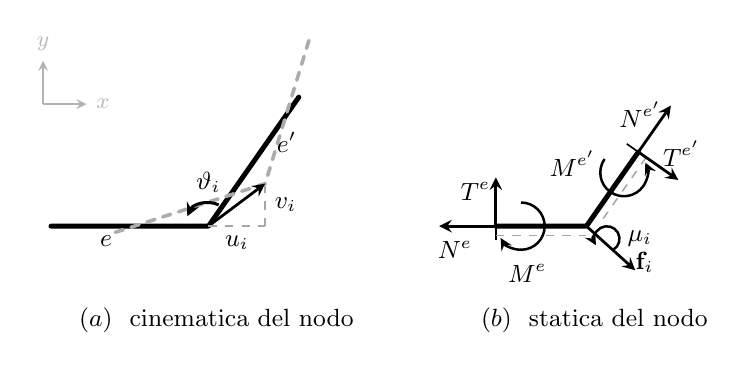
\begin{tikzpicture}[
			trave/.style={line width=1.8pt, line cap=round, line join=round, black},
			ghost/.style={line width=1.3pt, dashed, line cap=round, line join=round, gray!65},
			forza/.style={->, >=stealth, line width=1.0pt, black},
			momento/.style={->, >=stealth, line width=0.9pt, black},
			guida/.style={line width=0.55pt, dashed, gray!70},
			taglio/.style={line width=0.6pt, black},
			asse/.style={->, >=stealth, line width=0.6pt, gray!60},
			lab/.style={font=\small},
			labg/.style={font=\footnotesize, gray!55},
			]
			
			\def\Le{2.0}      % trave e (orizzontale, a sinistra del nodo)
			\def\Lep{2.0}     % trave e'
			\def\ang{55}      % inclinazione di e'  (angolo incluso ~125°)
			\def\SEP{4.8}     % separazione tra i pannelli
			
			%%═══ PANNELLO (a) — cinematica del nodo ══════════════════════════
			\begin{scope}
				% configurazione indeformata (spigolo rigido continuo, nessun cerchio)
				\draw[trave] (-\Le,0) -- (0,0) -- ({\Lep*cos(\ang)},{\Lep*sin(\ang)});
				% configurazione spostata: rigida = rotazione \rot attorno al nodo + traslazione (du,dv)
				\def\du{0.72}\def\dv{0.54}\def\rot{18}
				\begin{scope}[shift={(\du,\dv)}, rotate=\rot]
					\draw[ghost] (-\Le,0) -- (0,0) -- ({\Lep*cos(\ang)},{\Lep*sin(\ang)});
				\end{scope}
				% rotazione nodale, centrata sul nodo nella configurazione iniziale
				\draw[momento, line width=1.1pt] (0.13,0.27) arc (65:155:0.30);
				\node[lab, above] at (0,0.30) {$\vartheta_i$};
				% spostamento nodale e componenti nel riferimento globale
				\draw[forza] (0,0) -- (\du,\dv);
				\draw[guida] (0,0) -- (\du,0);
				\draw[guida] (\du,0) -- (\du,\dv);
				\node[lab, below] at ({\du/2},0) {$u_i$};
				\node[lab, right] at (\du,{\dv/2}) {$v_i$};
				% etichette travi
				\node[lab, below] at (-1.30,0) {$e$};
				\node[lab, right] at ({1.30*cos(\ang)},{1.30*sin(\ang)}) {$e'$};
				% assi globali
				\begin{scope}[shift={(-\Le-0.10,1.55)}]
					\draw[asse] (0,0) -- (0.55,0) node[labg, right] {$x$};
					\draw[asse] (0,0) -- (0,0.55) node[labg, above] {$y$};
				\end{scope}
				\node[lab] at (0.10,-1.20) {$(a)$ \ cinematica del nodo};
			\end{scope}
			
			%%═══ PANNELLO (b) — statica del nodo (corpo libero) ══════════════
			\begin{scope}[xshift=\SEP cm]
				\def\dc{1.15}   % posizione del taglio lungo ciascuna trave
				\def\nb{0.50}   % estensione del corpo-nodo lungo gli assi
				% corpo del nodo: materiale continuo (ombreggiato), non un perno
				%\fill[gray!15] (-\nb,0) -- (0,0) -- ({\nb*cos(\ang)},{\nb*sin(\ang)}) -- cycle;
				% tronconi isolati delle due travi
				\draw[trave] (-\dc,0) -- (0,0) -- ({\dc*cos(\ang)},{\dc*sin(\ang)});
				
				% ---- estremità della trave e (taglio a sinistra) ----
				\draw[taglio] (-\dc,-0.18) -- (-\dc,0.18);            % sezione
				\draw[guida]  (-\dc,-0.12) -- (-0.0,-0.12);          % lato fibre tese (tratteggio)
				\draw[forza]  (-\dc,0) -- (-\dc-0.72,0);              % N_e (trazione, uscente)
				\node[lab] at (-\dc-0.52,-0.30) {$N^e$};
				\draw[forza]  (-\dc,0) -- (-\dc,0.62);                % T_e (trasversale, verso l'alto)
				\node[lab] at (-\dc-0.26,0.44) {$T^e$};
				%				\draw[forza]  (-\dc,0) -- (-\dc,-0.62);               % T_e (trasversale)
				%				\node[lab] at (-\dc-0.26,-0.44) {$T_e$};
				\draw[momento] (-\dc+0.32,0.30) arc (90:-150:0.30);   % M_e
				\node[lab] at (-\dc+0.40,-0.60) {$M^e$};
				
				% ---- estremità della trave e' (taglio in alto a destra) ----
				\begin{scope}[shift={({\dc*cos(\ang)},{\dc*sin(\ang)})}, rotate=\ang]
					\draw[taglio] (0,-0.18) -- (0,0.18);              % sezione
					\draw[guida]  (0,-0.12) -- (-1.05,-0.12);         % lato fibre tese
					\draw[forza]  (0,0) -- (0.72,0);                  % N_{e'} (trazione, uscente)
					\node[lab] at (0.40,0.25) {$N^{e'}$};
					\draw[forza]  (0,0) -- (0,-0.62);                 % T_{e'} (invertito)
					\node[lab] at (0.30,-0.46) {$T^{e'}$};
					
					
					%					\draw[forza]  (0,0) -- (0,0.62);                  % T_{e'}
					%					\node[lab] at (0.30,0.46) {$T_{e'}$};
					\draw[momento] (-0.32,0.30) arc (90:330:0.30);    % M_{e'}
					\node[lab] at (-0.60,0.60) {$M^{e'}$};
				\end{scope}
				
				% carichi nodali esterni (eventuali): forza \fb_i e coppia \mu_i
				\draw[forza] (0,0) -- (0.62,-0.56);
				\node[lab, right] at (0.50,-0.46) {$\mathbf{f}_i$};
				\draw[momento] (0.34,-0.30) arc (-60:210:0.16);
				\node[lab, right] at (0.40,-0.16) {$\mu_i$};
				
				\node[lab] at (0.10,-1.20) {$(b)$ \ statica del nodo};
			\end{scope}
			
		\end{tikzpicture}
	}%
	\caption{Nodo rigido tra due travi, $e$ ed $e'$. A sinistra:
		cinematica del nodo --- le tre componenti di spostamento
		nodale $(u_i, v_i, \vartheta_i)$ nel riferimento globale,
		condivise da entrambe le travi, che ruotano rigidamente
		conservando l'angolo. A destra: statica del nodo isolato
		come corpo libero --- le caratteristiche di estremità
		$N$, $T$, $M$ trasmesse da ciascuna trave, riferite al
		rispettivo sistema locale (lato delle fibre tese a
		tratteggio), e gli eventuali carichi nodali esterni ---
		forza $\mathbf{f}_i$ e coppia $\mu_i$ ---, in equilibrio
		al nodo: $\sum\mathbf{f}=\mathbf{0}$, $\sum \mu= 0$.}
	\label{fig:nodo_rigido}
\end{figure}
